\section{Appendix}

\subsection{Related Work Visual References}

\begin{figure}[htbp]
  \centering
  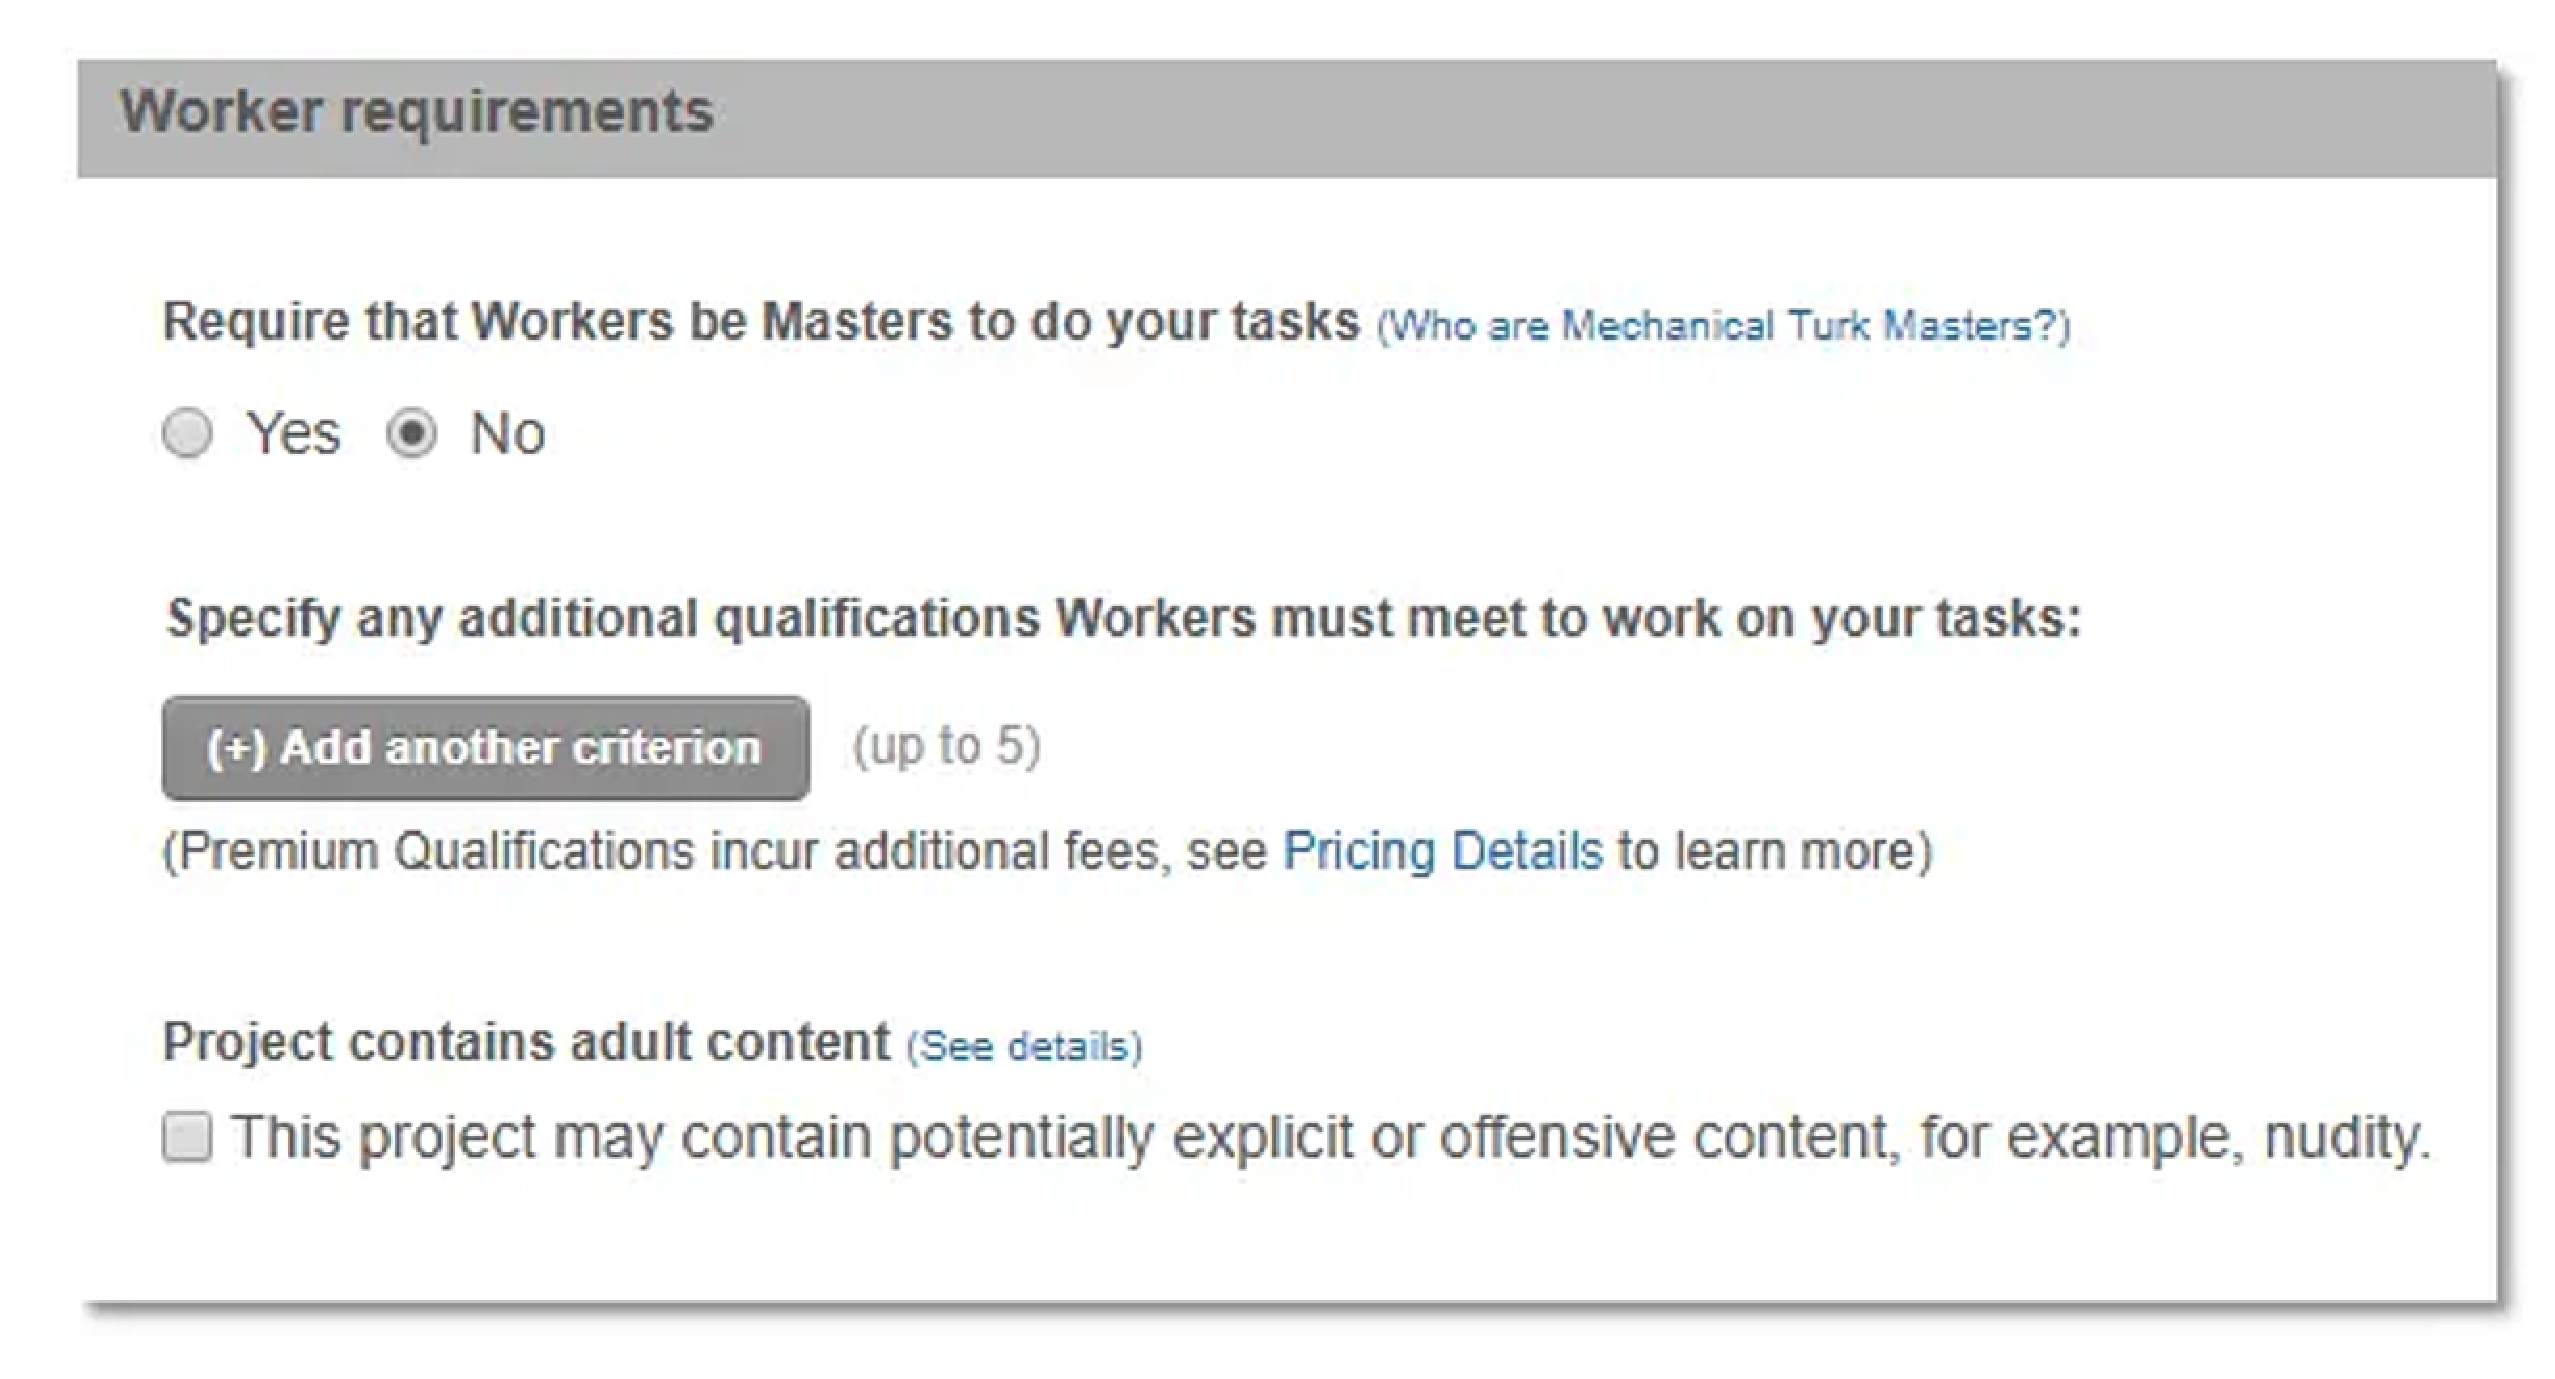
\includegraphics[width=\linewidth]{figures/mturk_adult_qualification.pdf}
  \caption{MTurk’s adult content qualification requirement for screening workers.}
  \label{fig:mturk_adult}
\end{figure}

\begin{figure}[htbp]
    \centering
    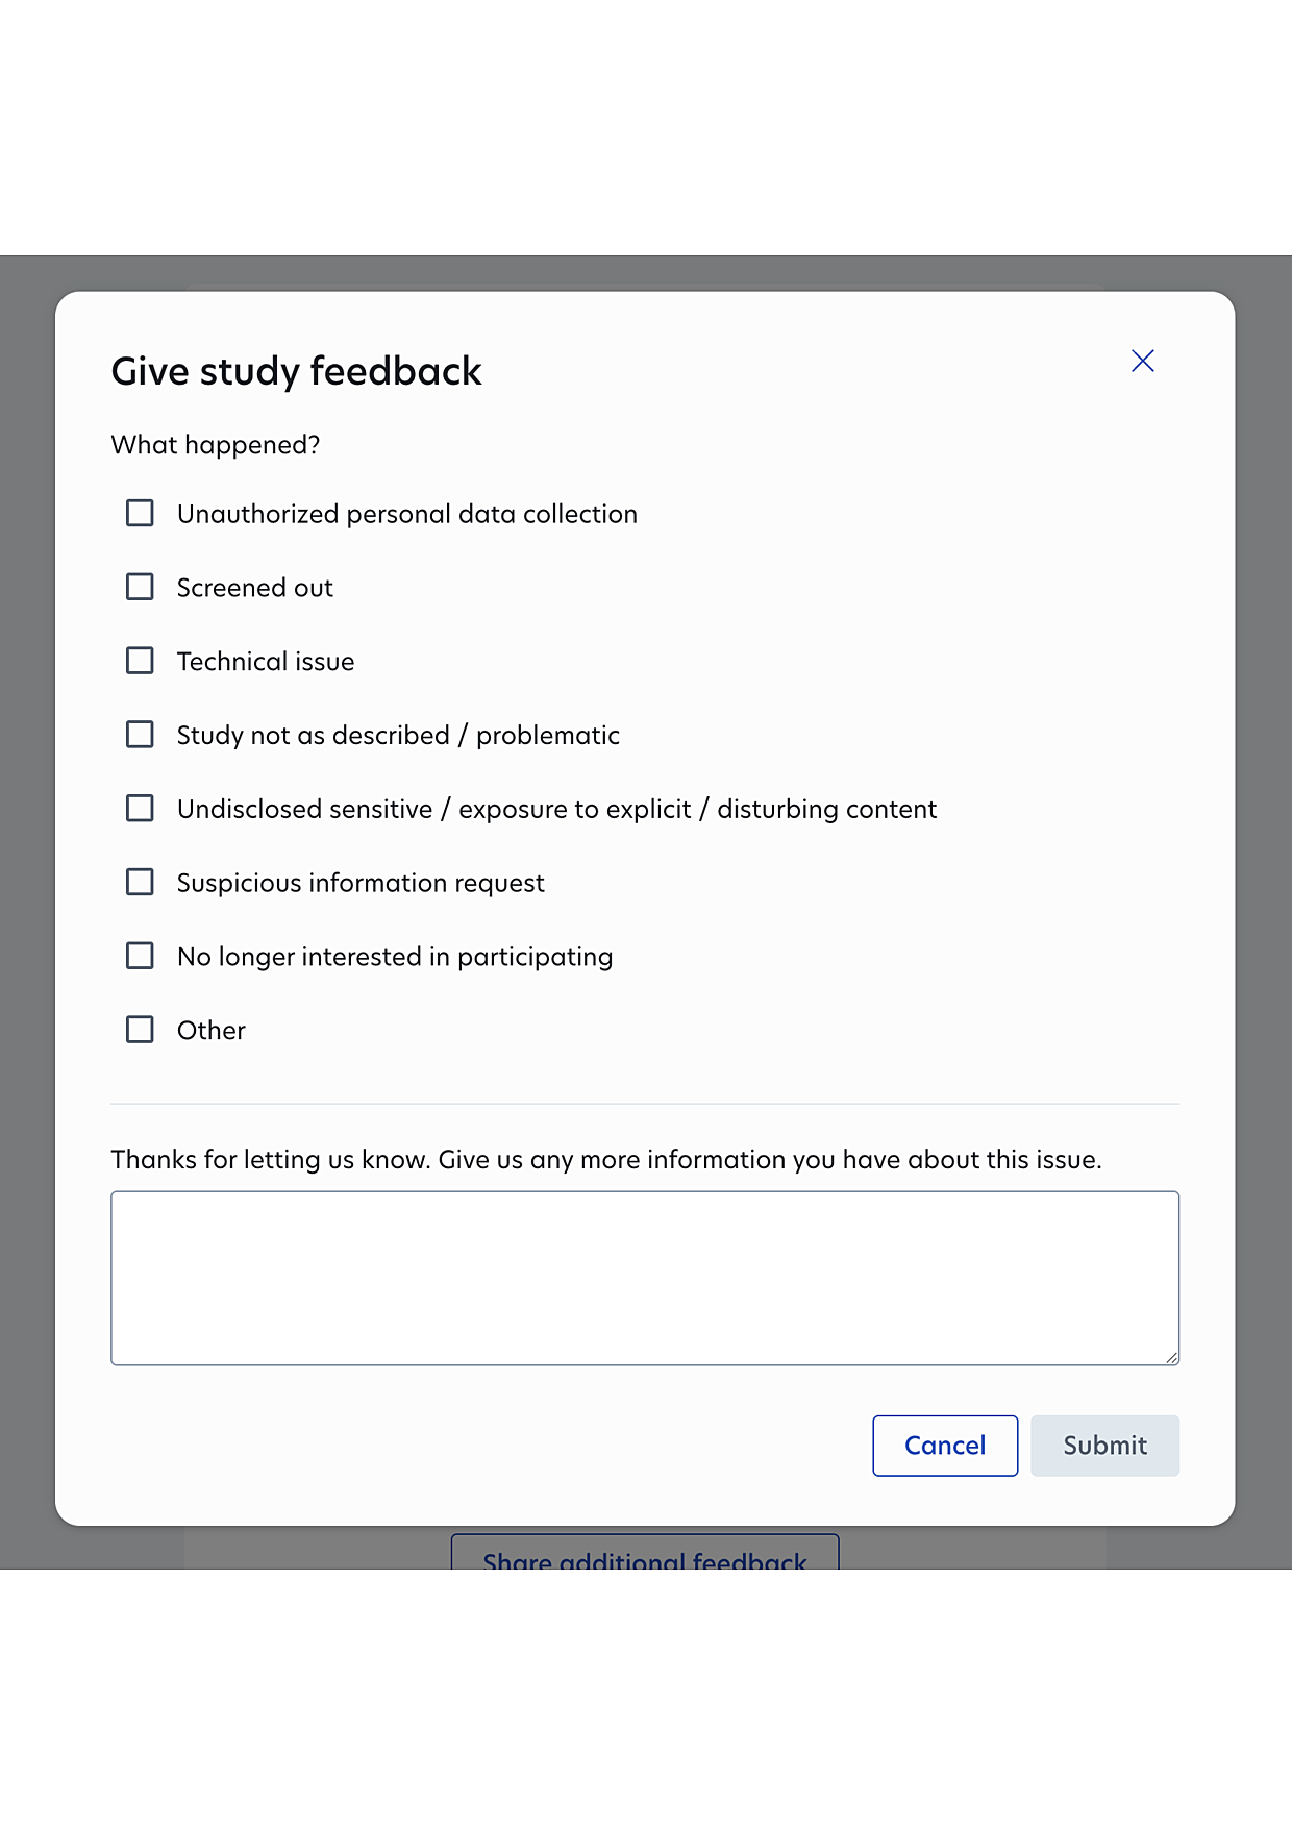
\includegraphics[width=\columnwidth]{figures/prolific_feedback_extra.pdf}
    \caption{Option to provide extra feedback on Prolific}
    \label{fig:prolific-feedback-extra}
\end{figure}

\begin{figure}[htbp]
    \centering
    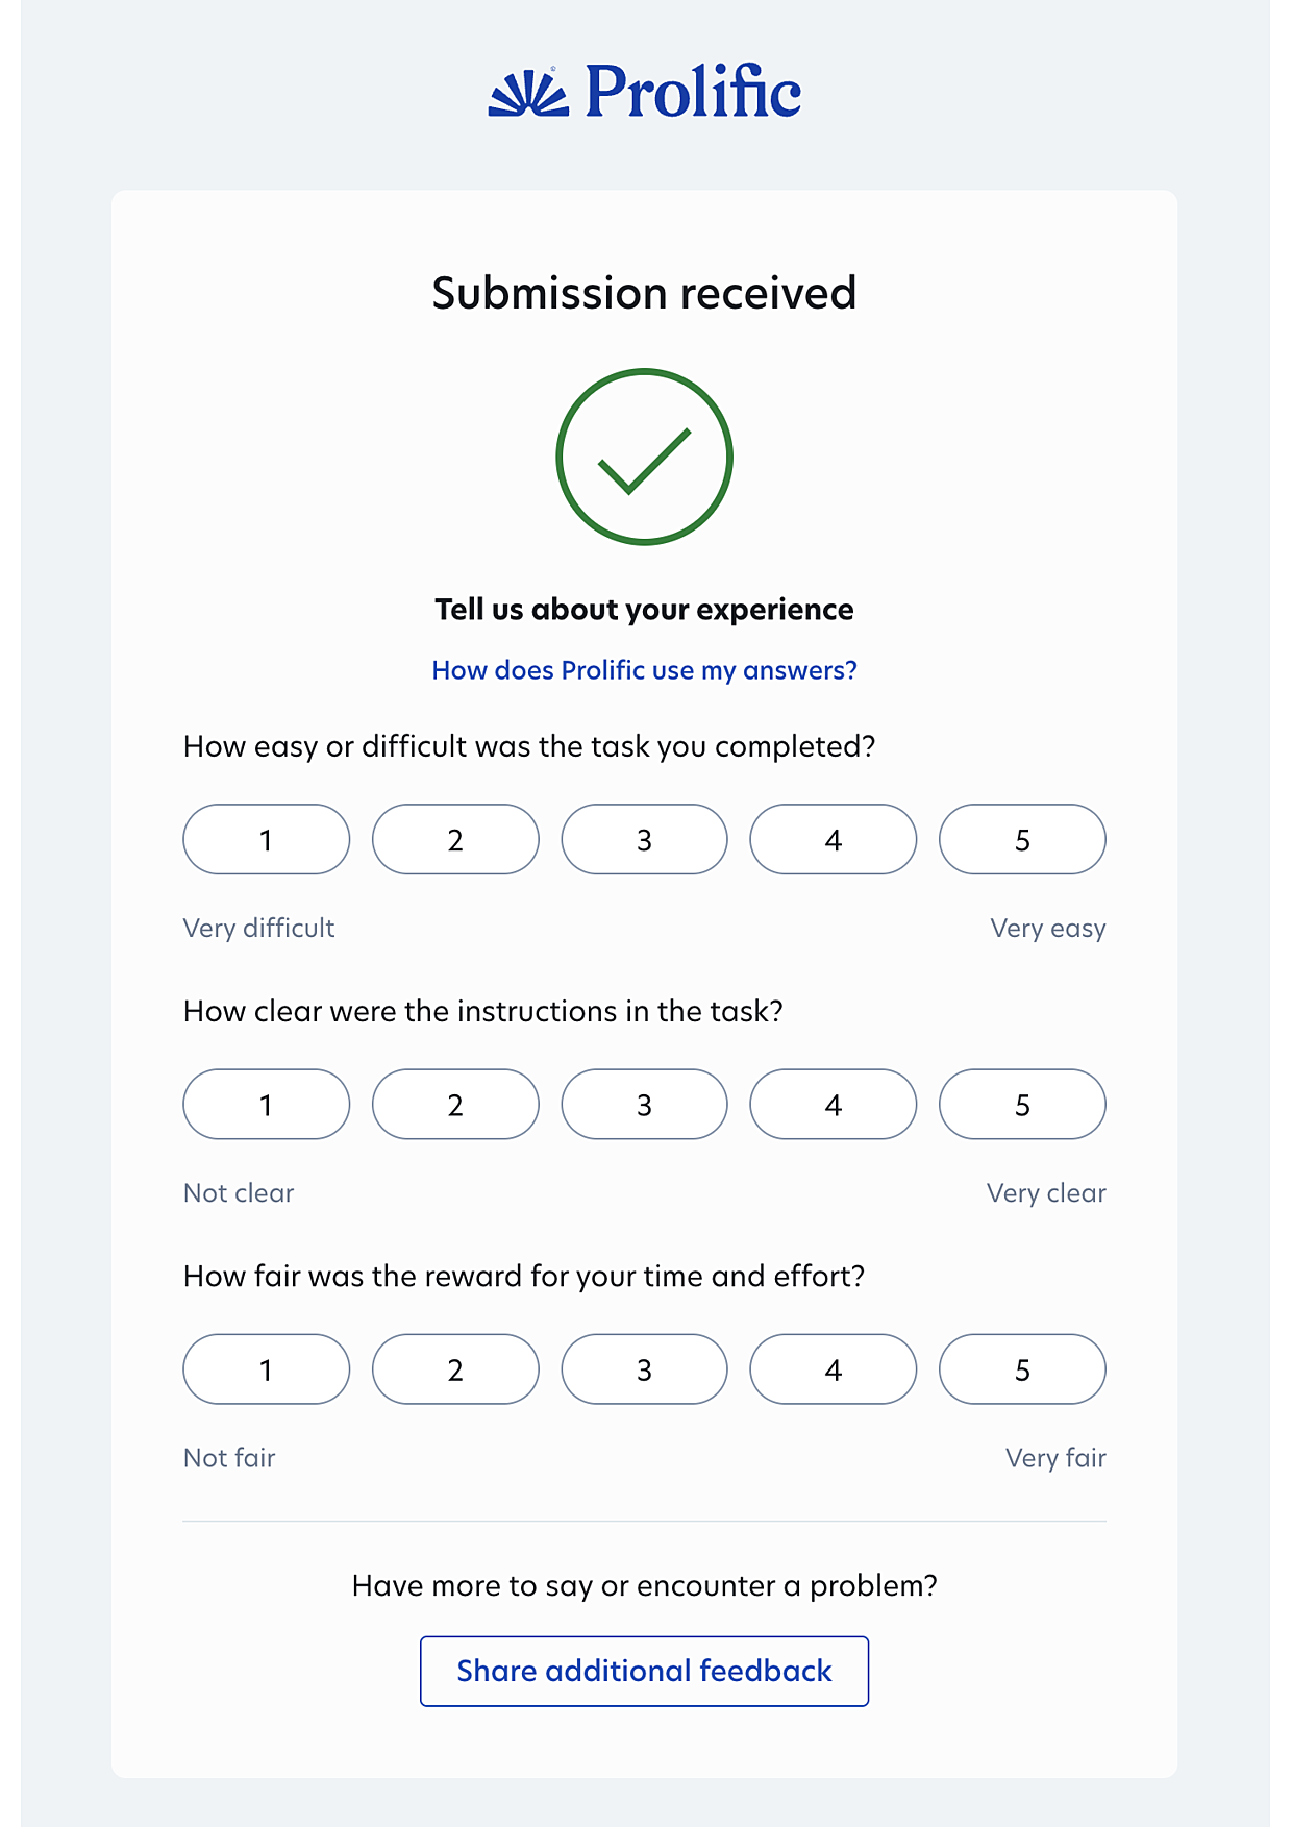
\includegraphics[width=\columnwidth]{figures/prolific_feedback.pdf}
    \caption{Option to provide feedback on Prolific}
    \label{fig:prolific-feedback}
\end{figure}


\begin{figure}[htbp]
    \centering
    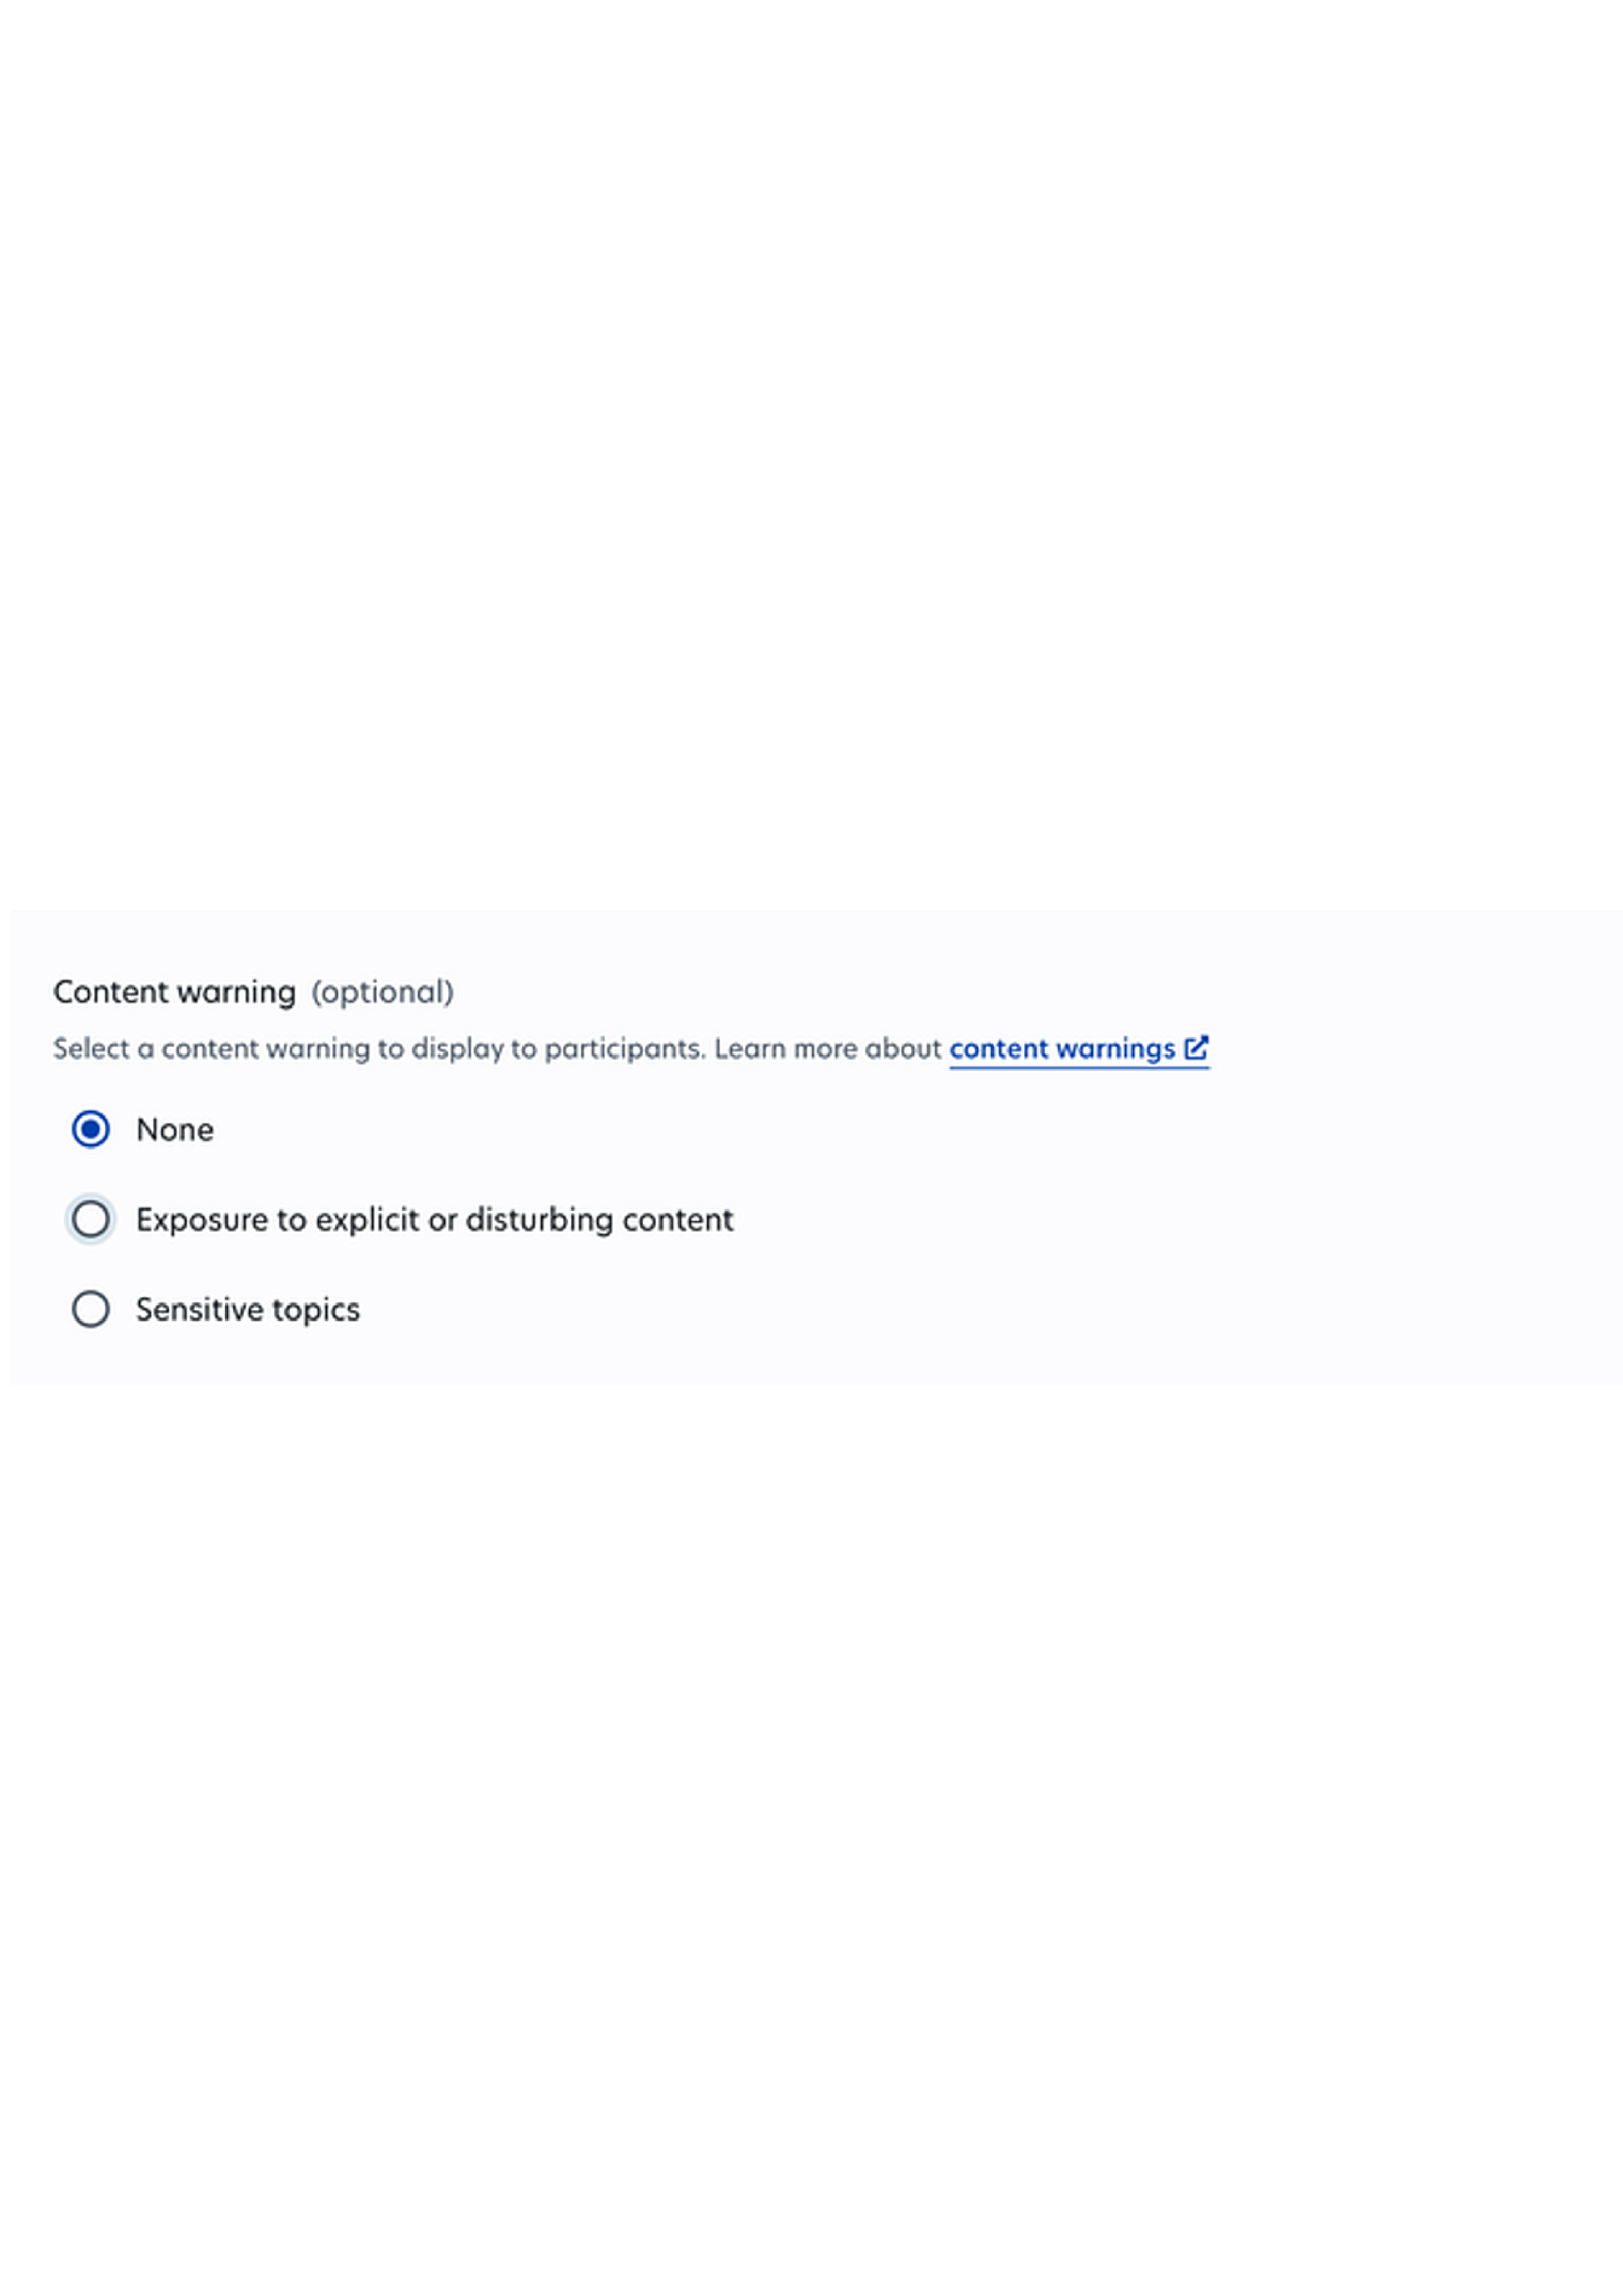
\includegraphics[width=\columnwidth]{figures/prolific_zoomedin_binary.pdf}
    \caption{Close-up of the sensitive content warning presented to workers.}
    \label{fig:prolific_zoomed}
\end{figure}

\begin{figure}[H]
    \centering
    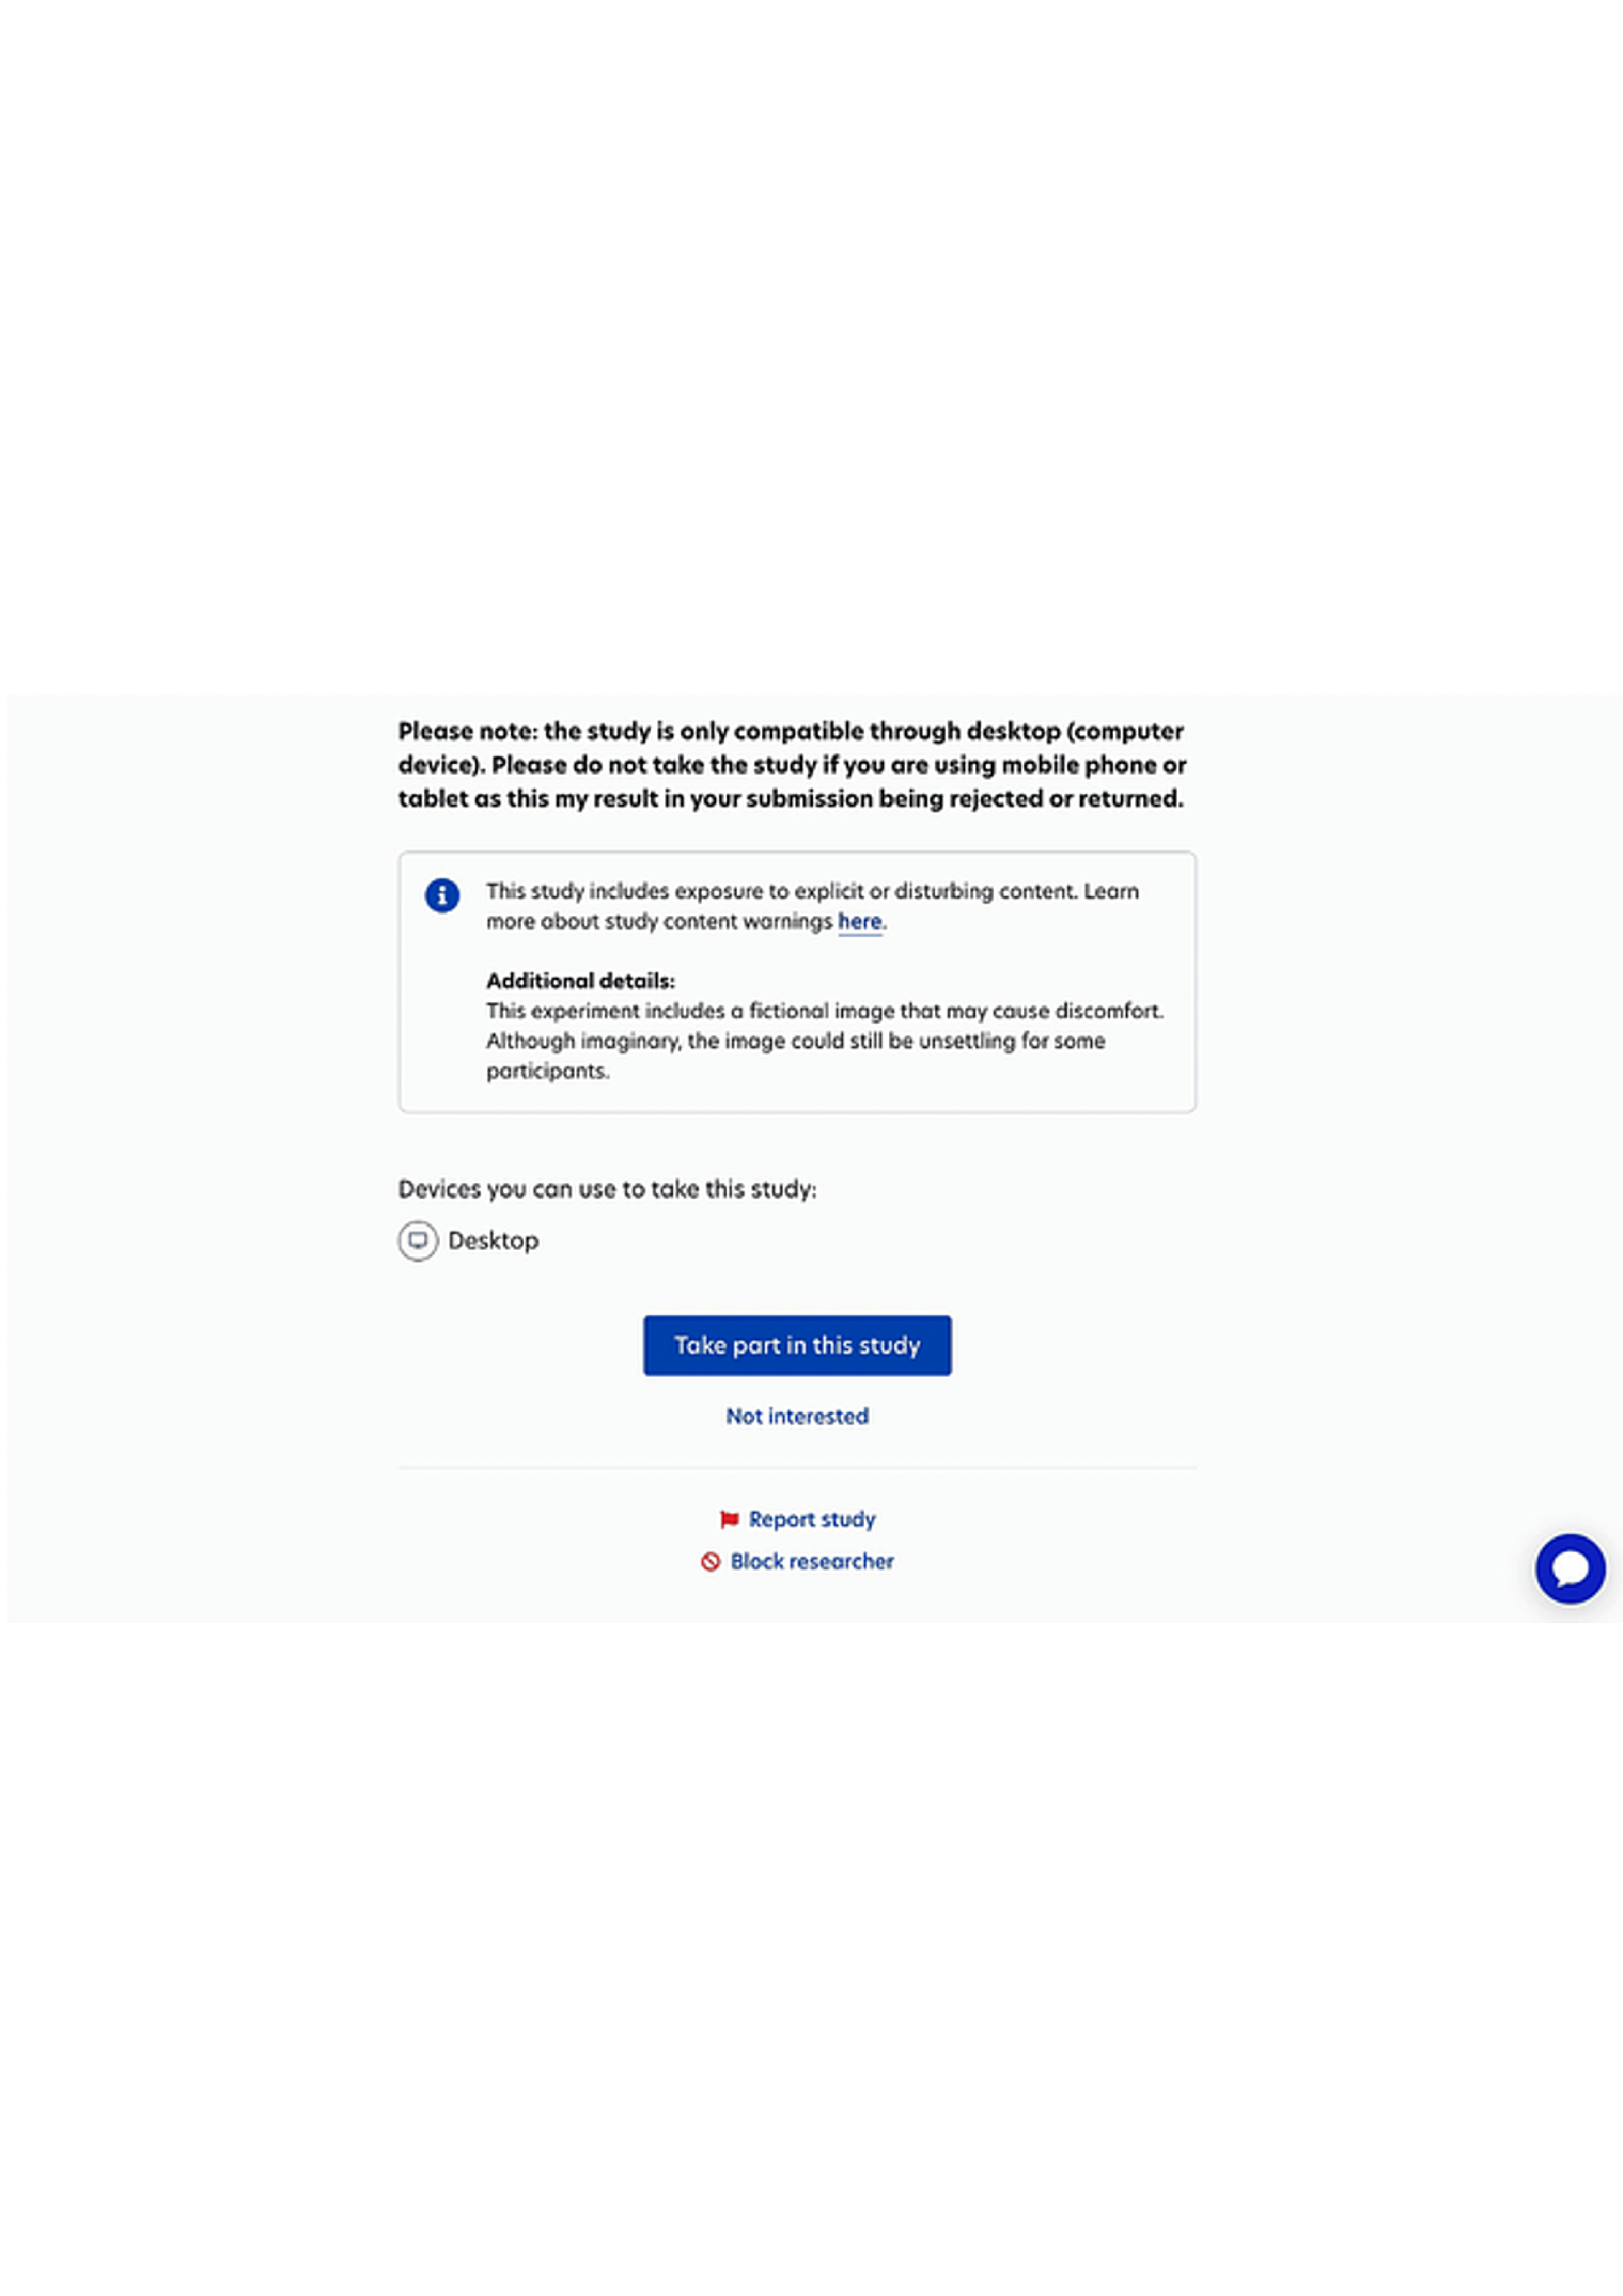
\includegraphics[width=\columnwidth]{figures/prolific_worker_side_example.pdf}
    \caption{Worker-facing task list view with a sensitive content label.}
    \label{fig:prolific_worker}
\end{figure}
\begin{figure} 
  \centering
  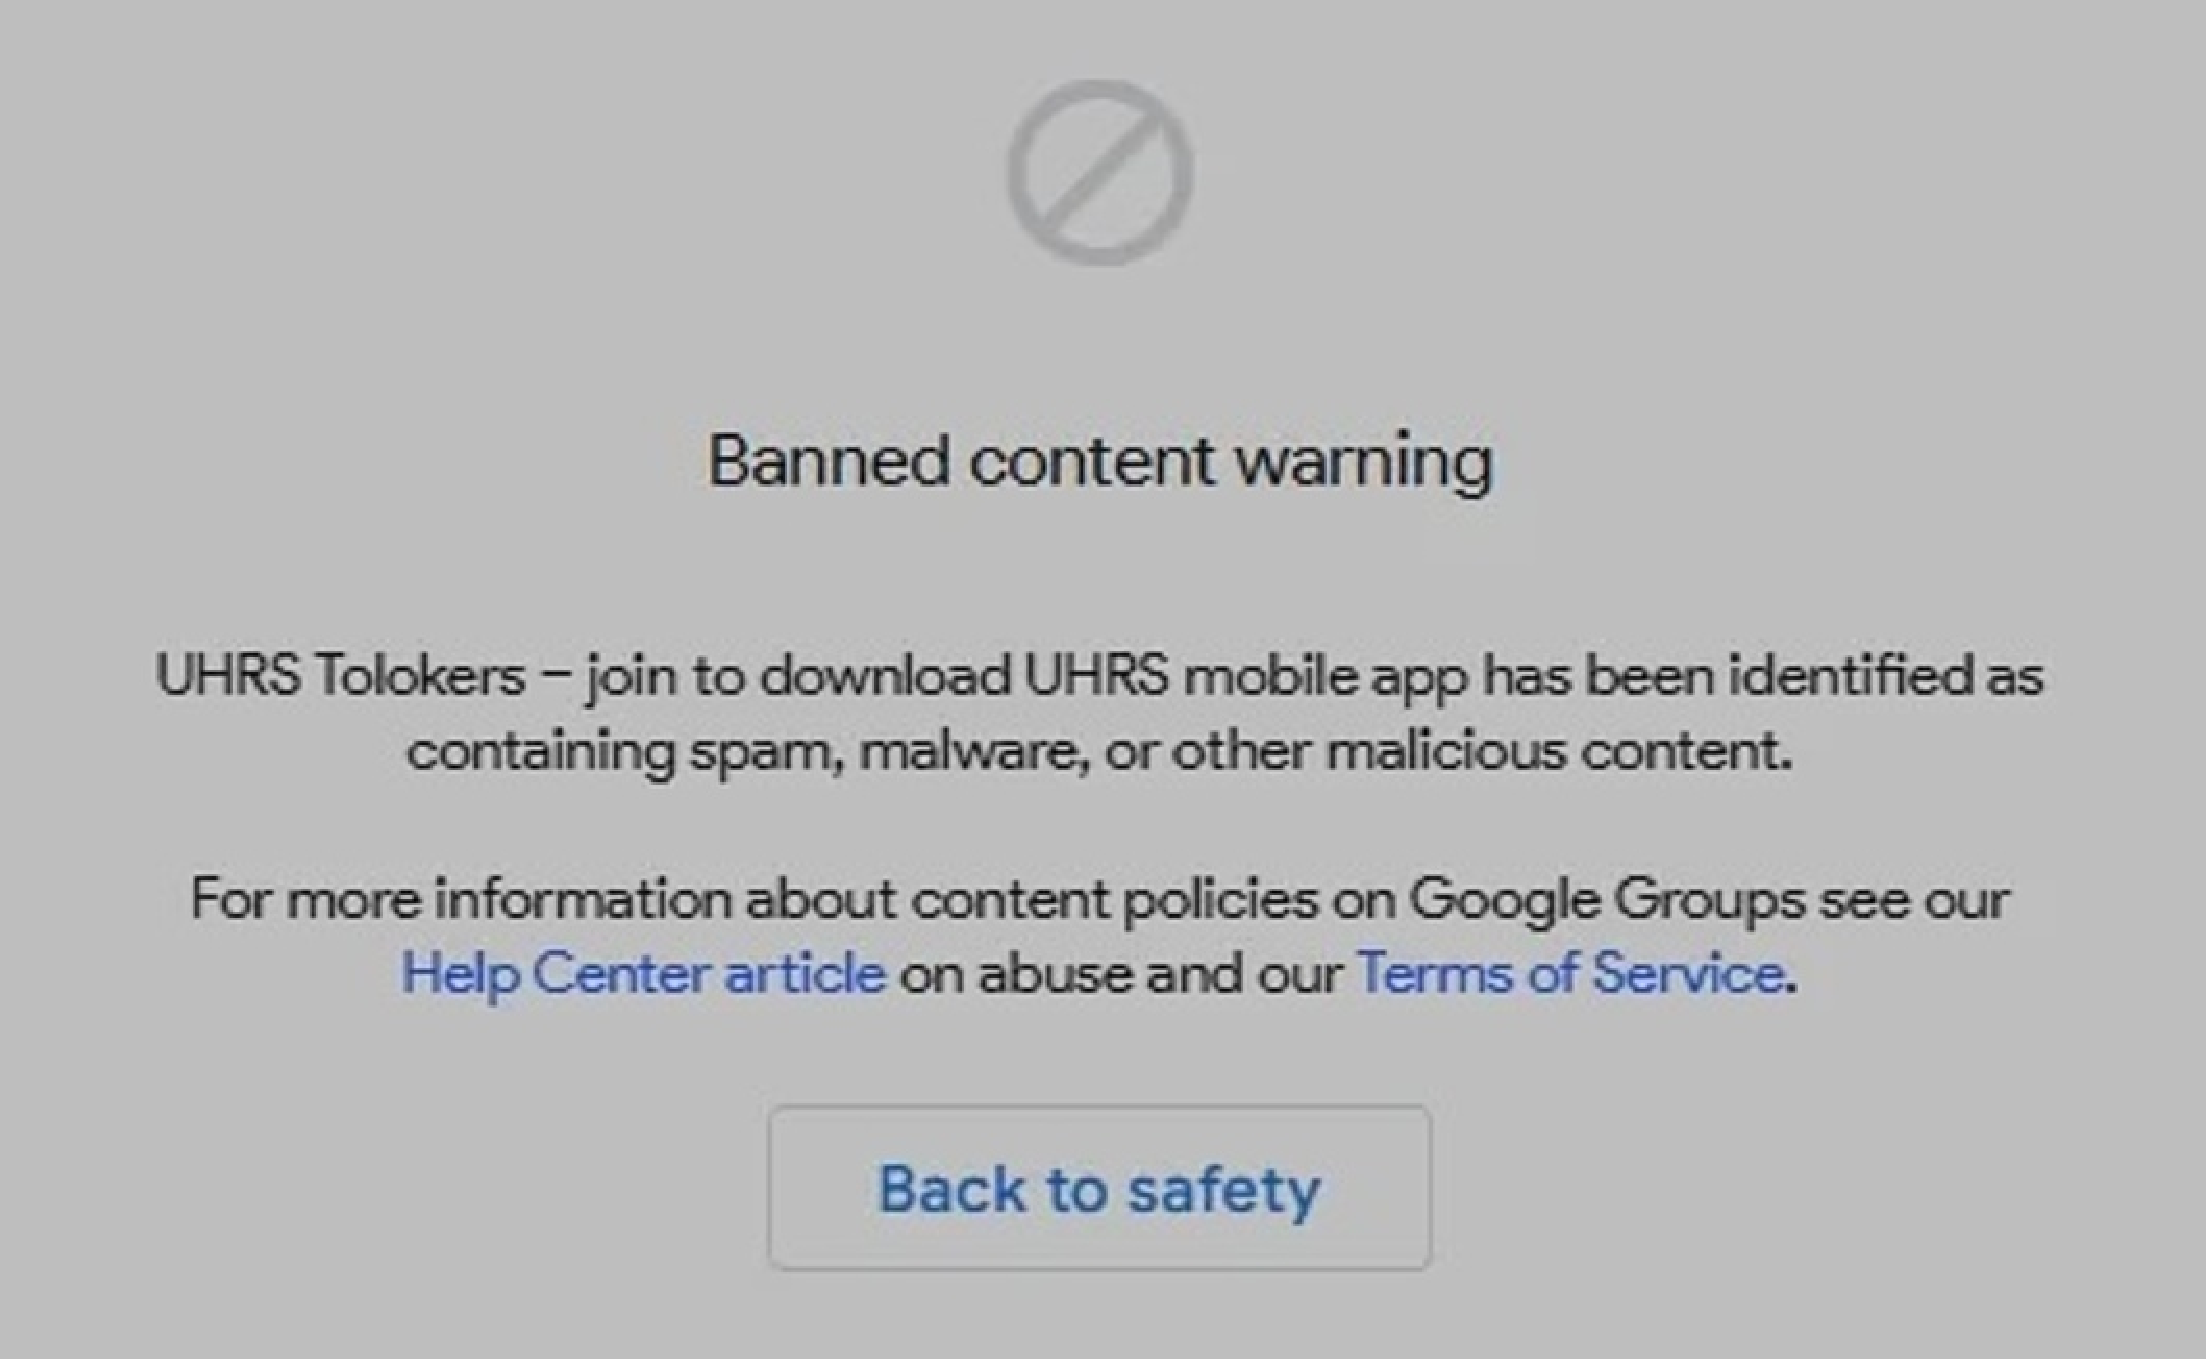
\includegraphics[width=0.7\linewidth]{figures/toloka_removed_task.pdf}
  \caption{Removed task page from Toloka, demonstrating limited access to past sensitive content.}
  \label{fig:toloka_removed}
\end{figure}


\begin{figure}[H]
  \centering
  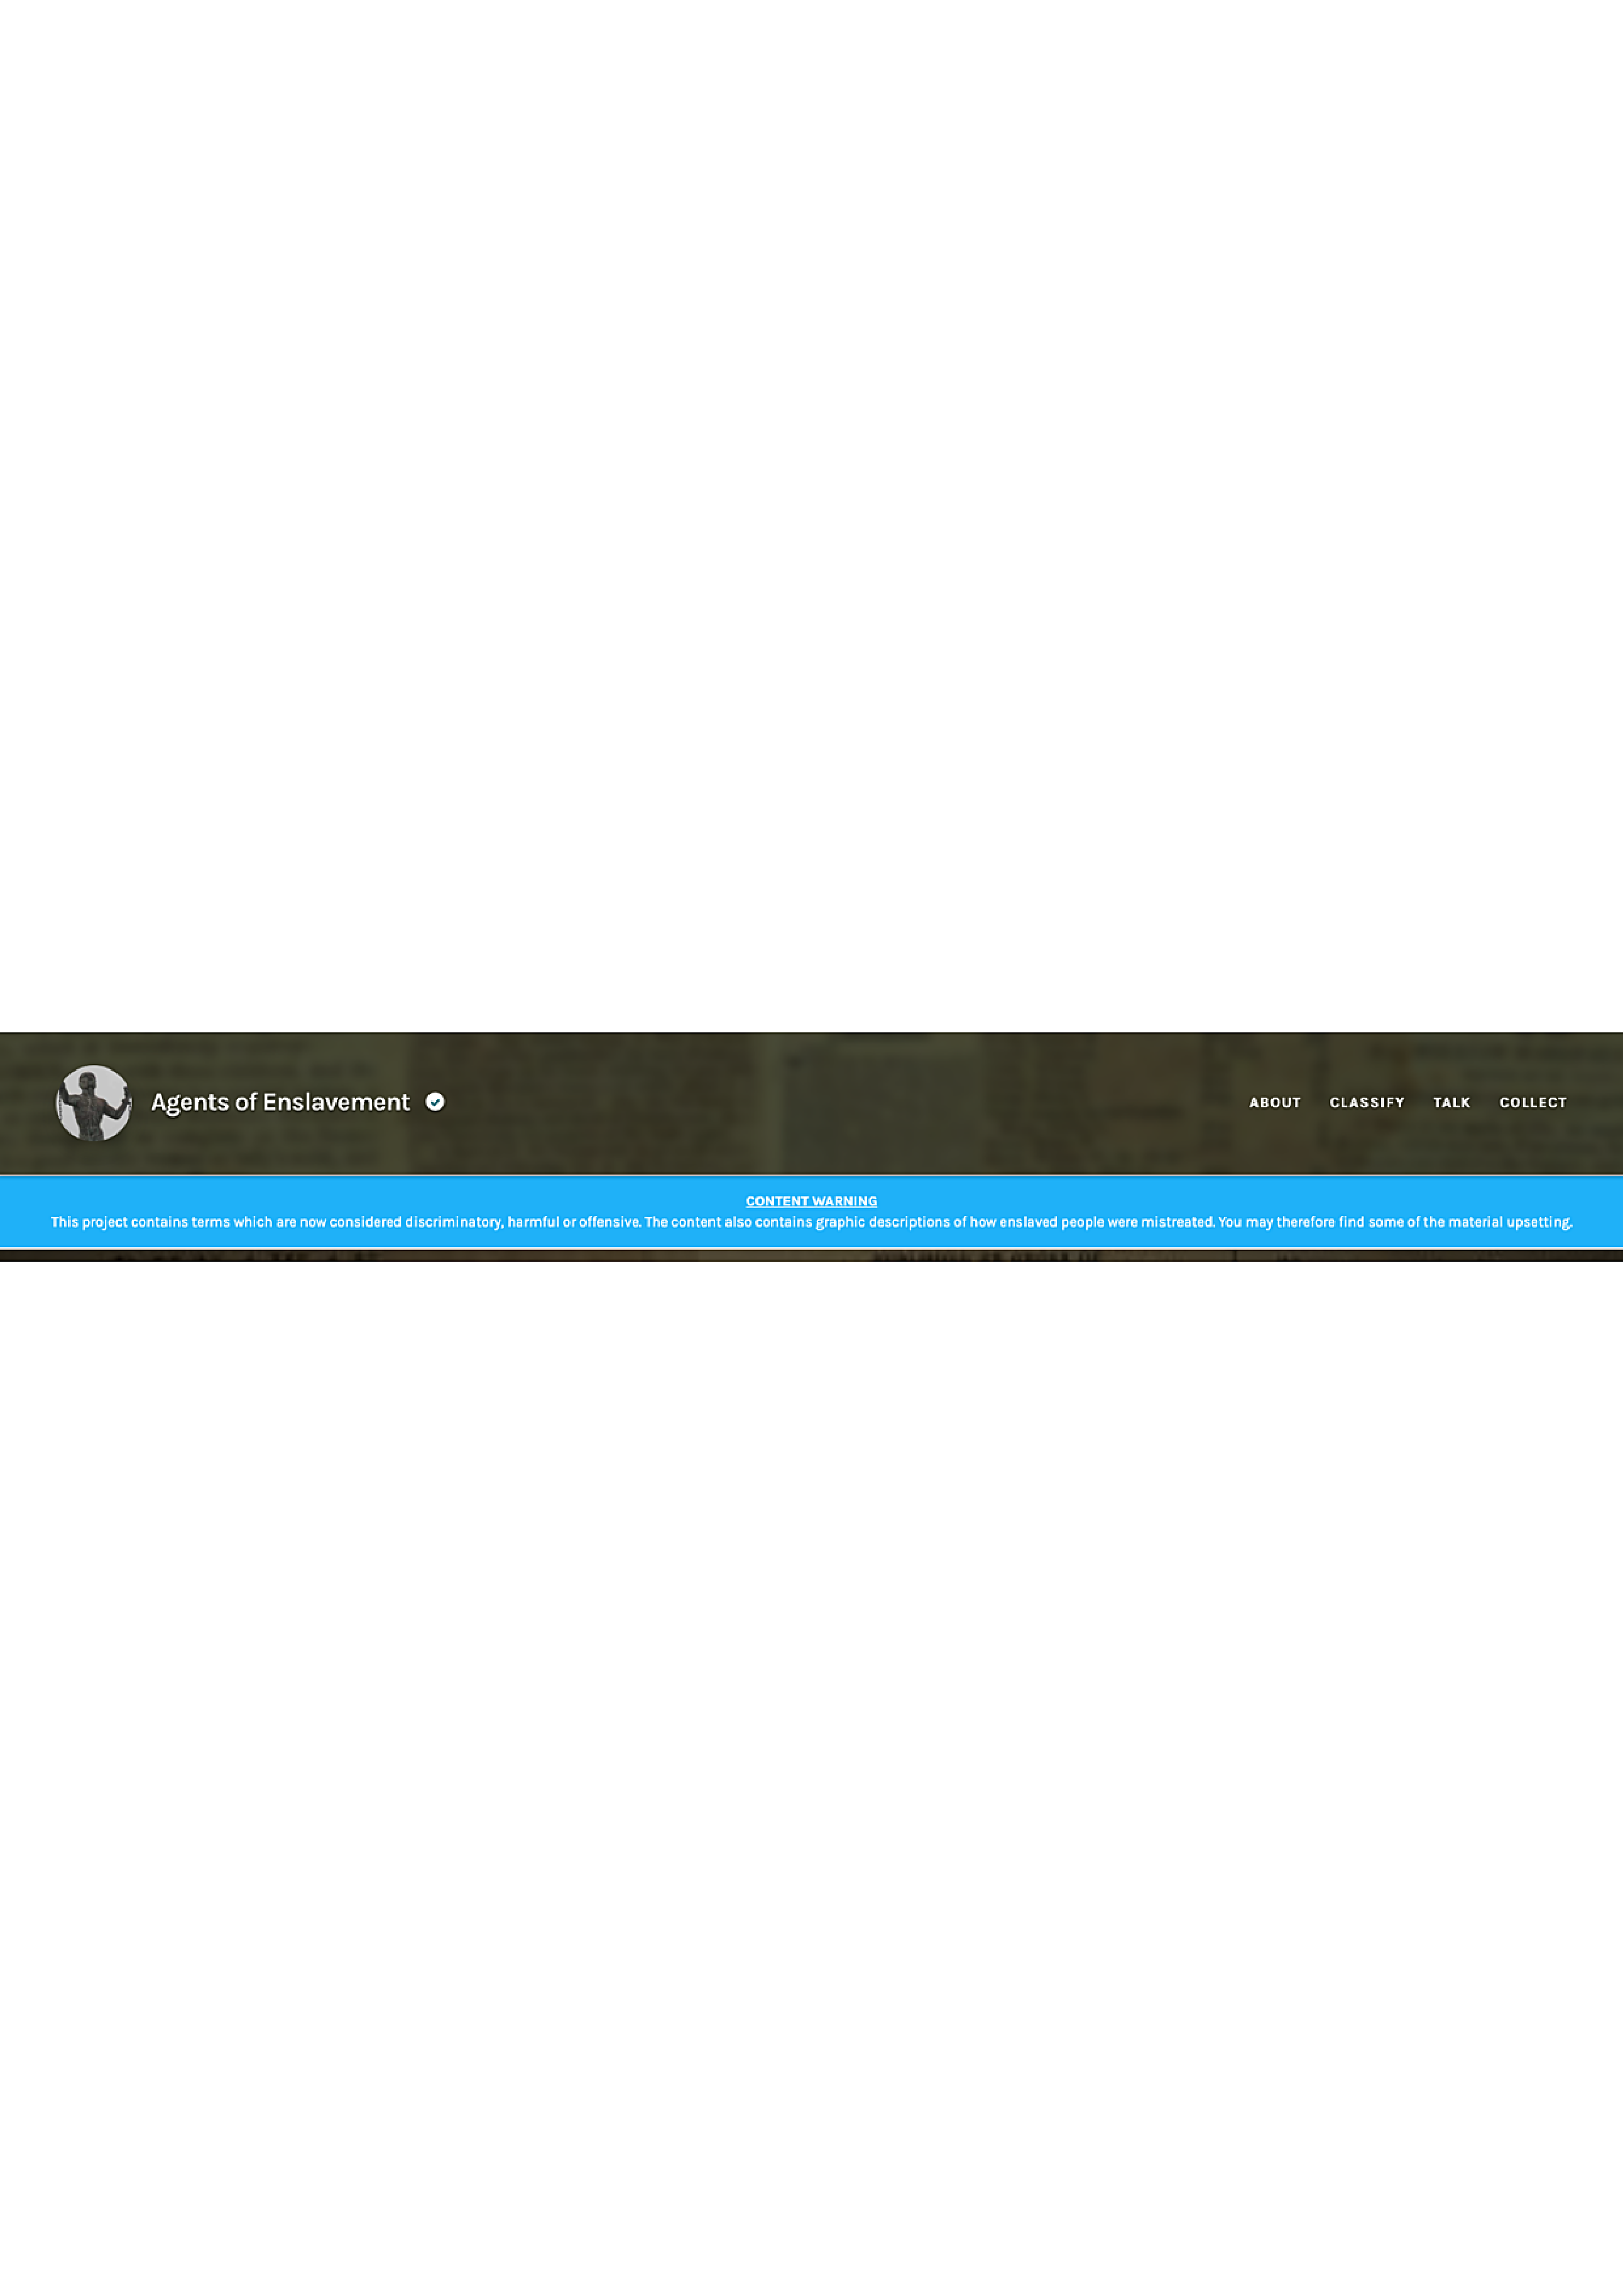
\includegraphics[width=\linewidth]{figures/warning_zooniverse.pdf}
  \caption{Task content warning from Zooniverse}
  \label{fig:zooniverse_removed}
\end{figure}







\subsection{Examples of Co-Design Probes}


\begingroup
\begin{figure}[H]
    \centering
    \begin{subfigure}[b]{0.48\textwidth}
        \centering
        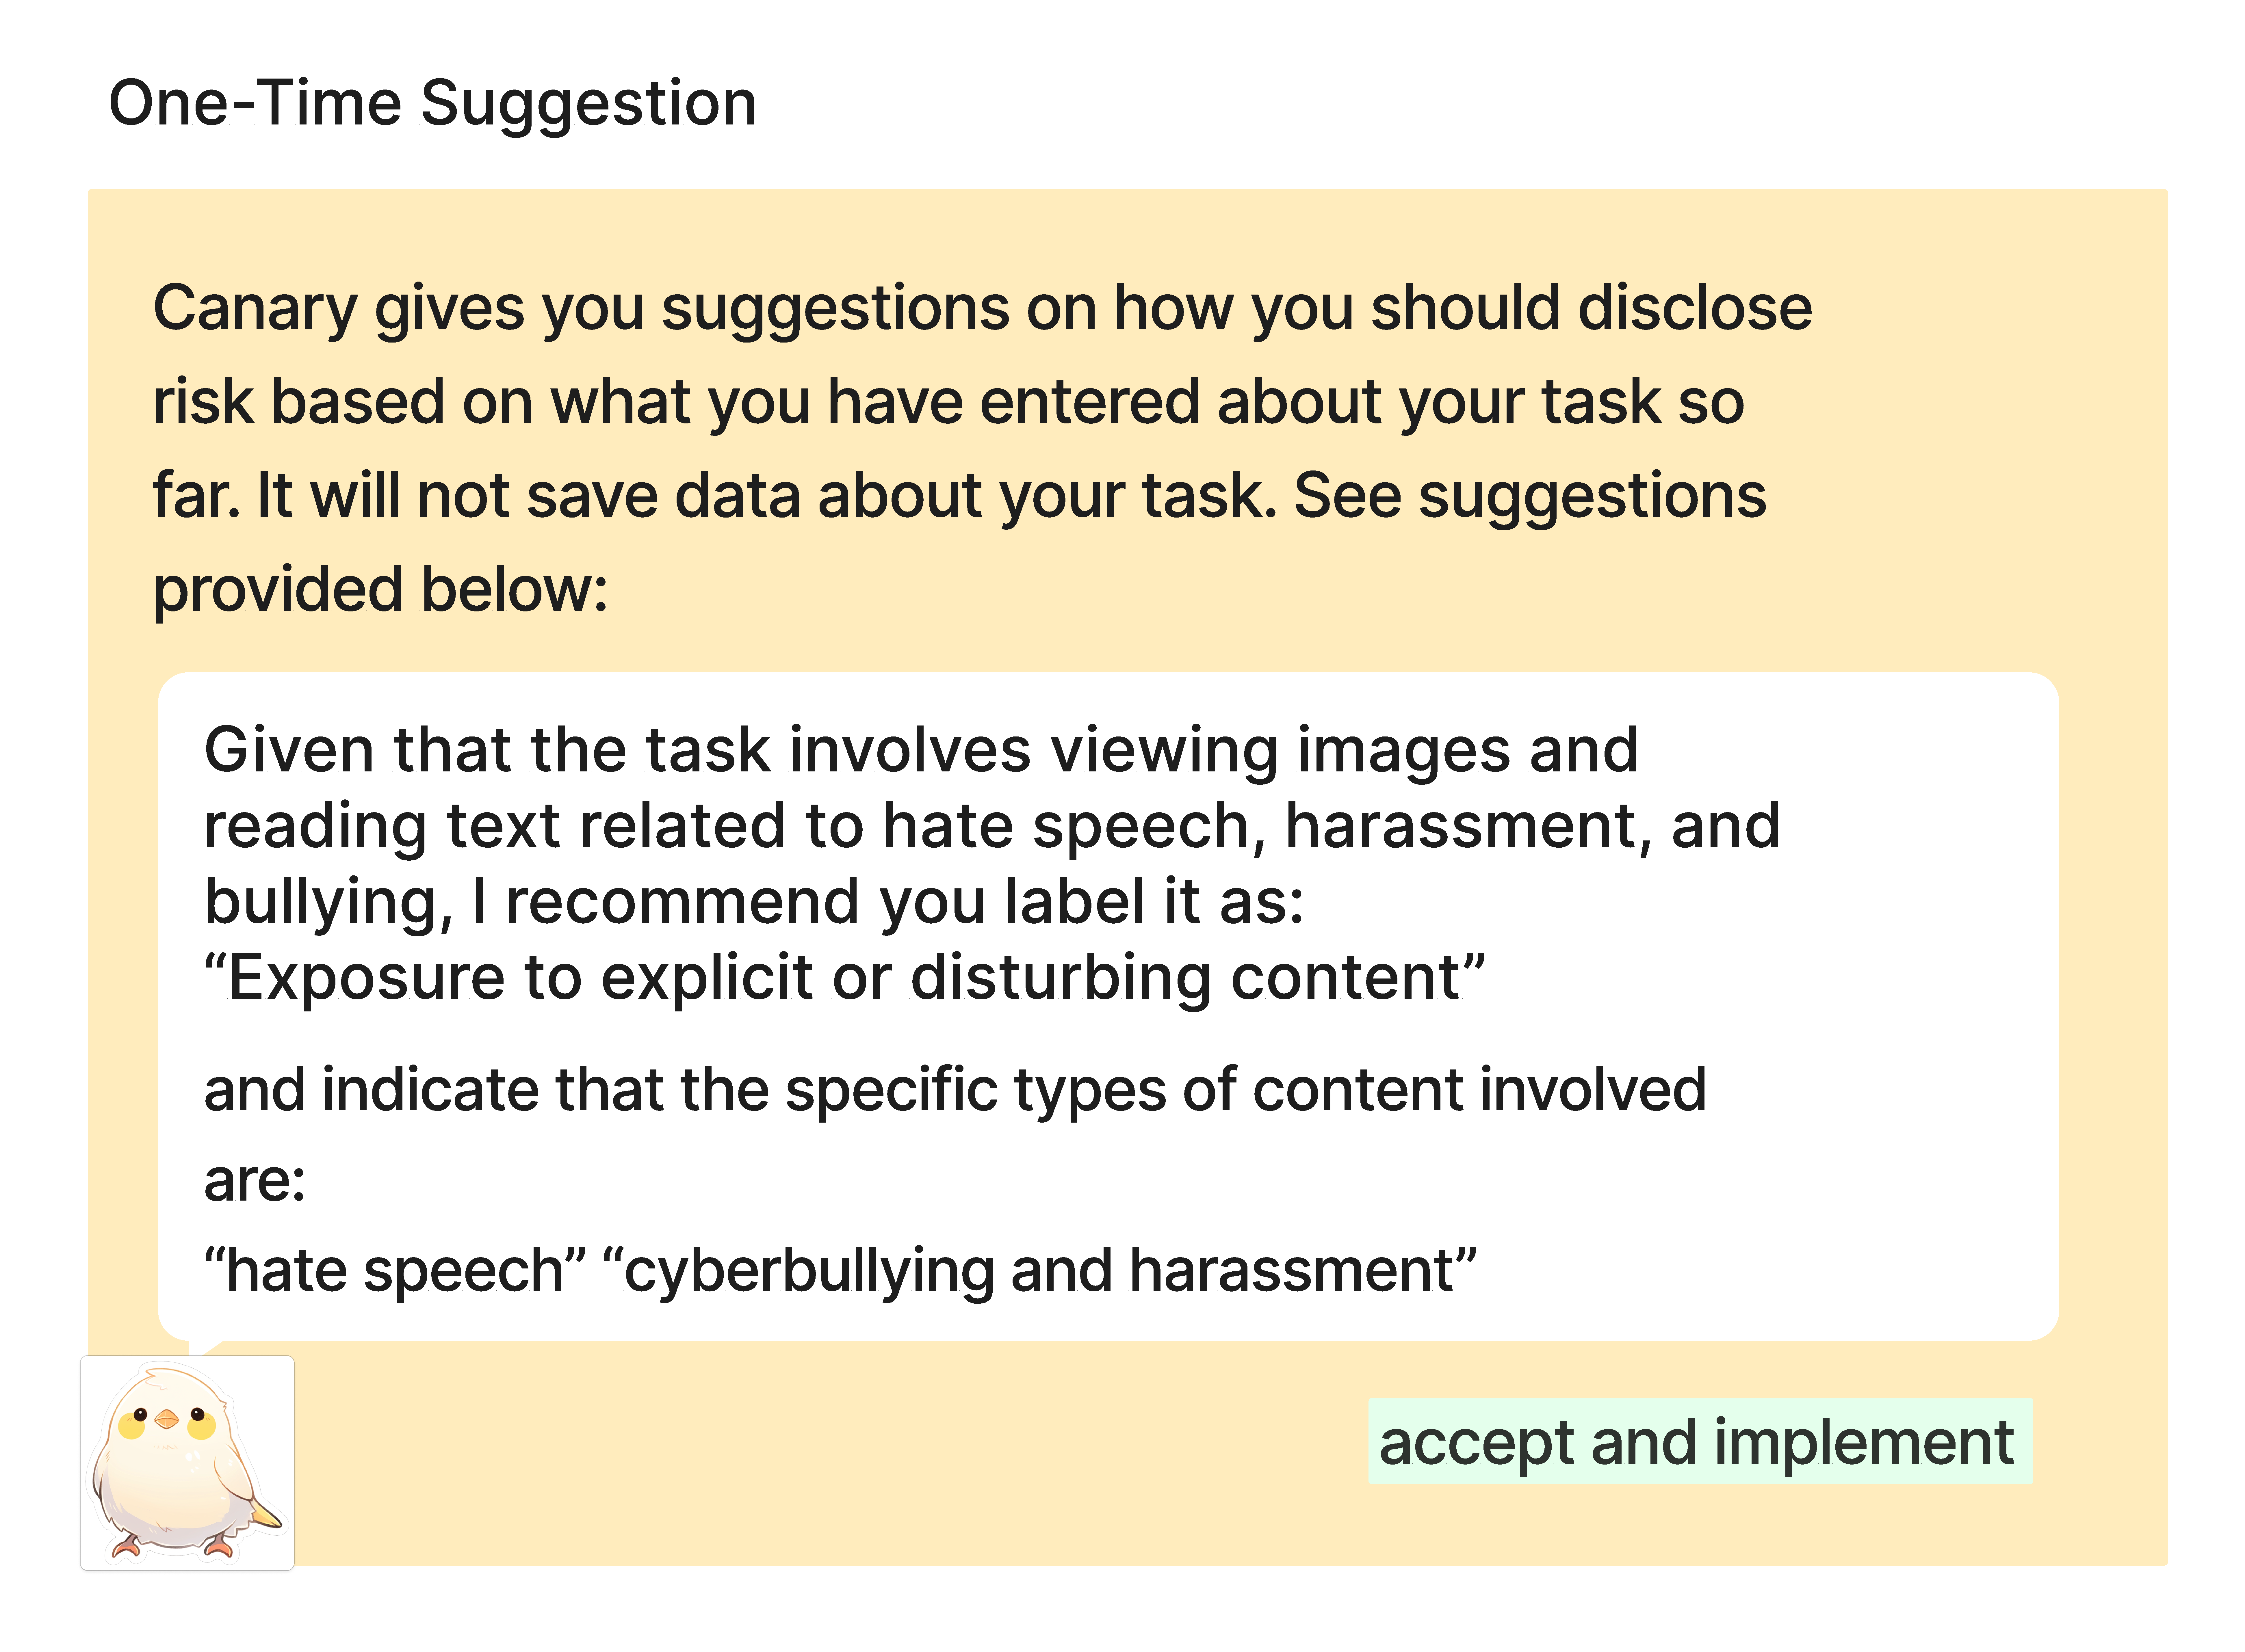
\includegraphics[width=\textwidth]{figures/study-probes/AI-probes/AI-one-time.pdf}
        \caption{Generic AI suggestion\protect\footnotemark}
        \label{fig:AI-generic}
    \end{subfigure}
    \hfill
    \begin{subfigure}[b]{0.48\textwidth}
        \centering
        \includegraphics[width=\textwidth]{figures/study-probes/AI-probes/AI-explanation.pdf} 
        \caption{AI suggestion with explanation}
        \label{fig:AI-explanation}
    \end{subfigure}
    \caption{AI warning suggestions (Part 1)}
    \label{fig:task-designer-AI-1}
\end{figure}

\begin{figure}[H]
    \centering
    \begin{subfigure}[b]{0.48\textwidth}
        \centering
        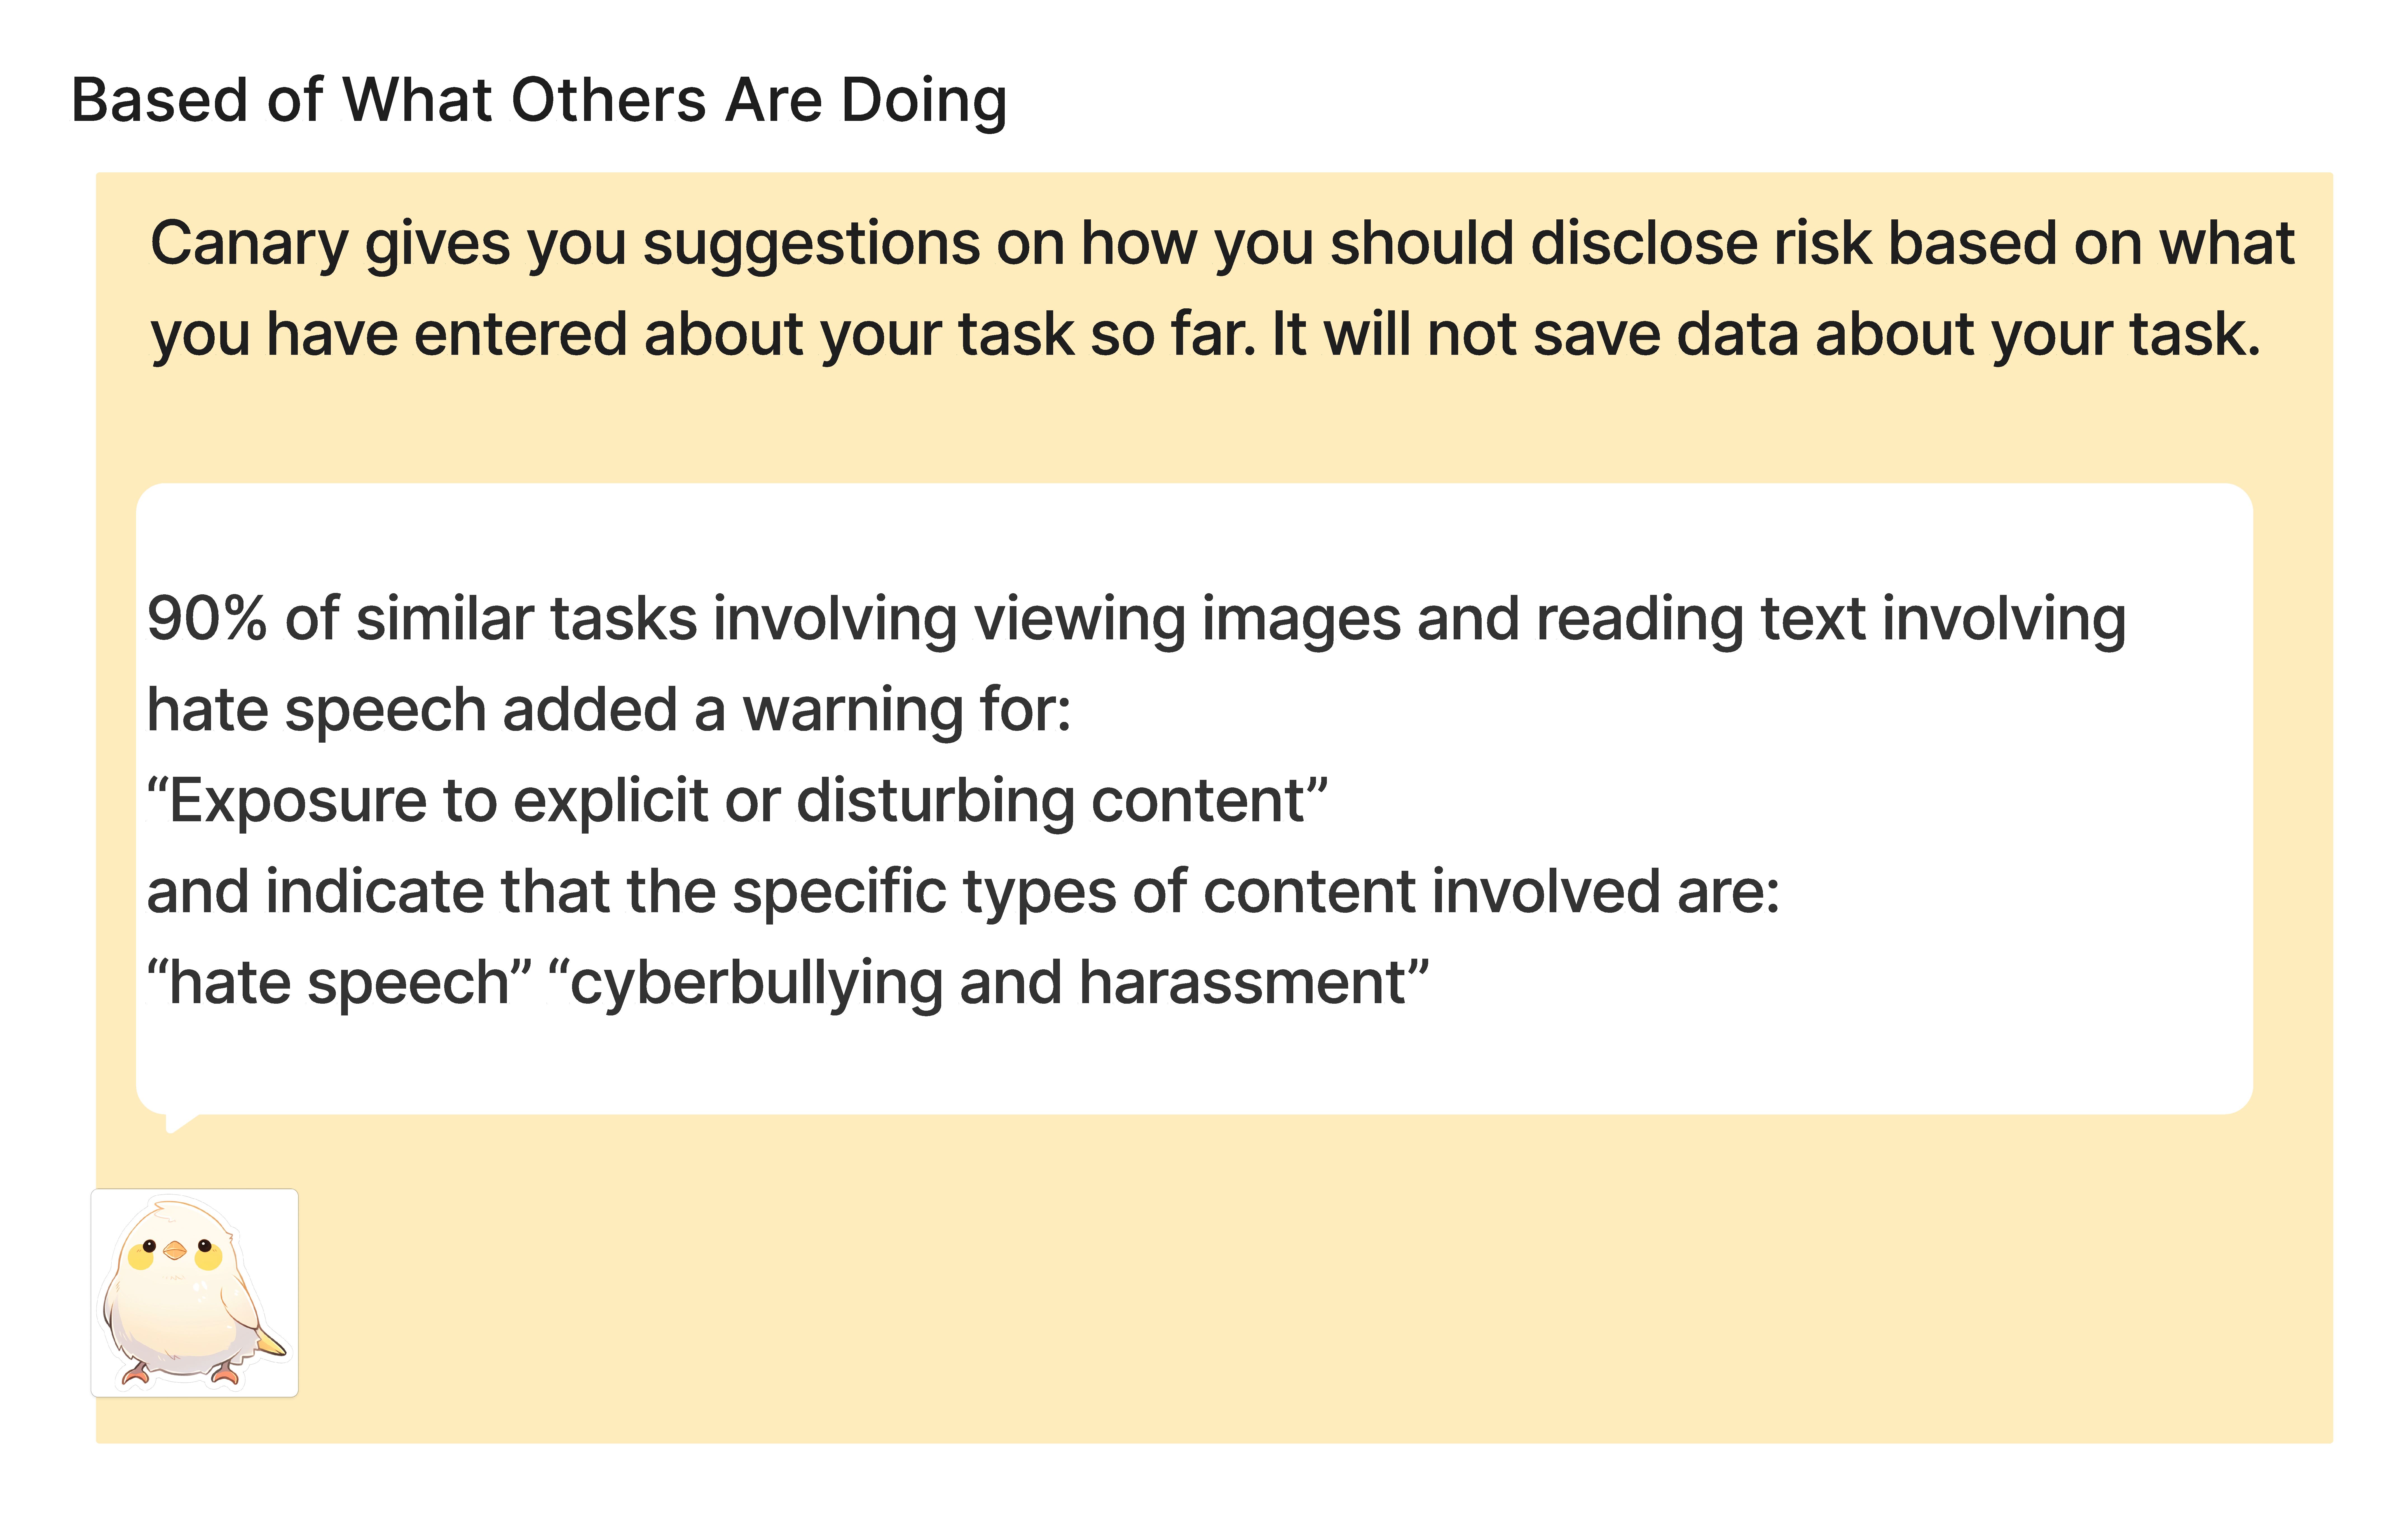
\includegraphics[width=\textwidth]{figures/study-probes/AI-probes/AI-task-designers.pdf}
        \caption{Suggestion based on what other task designers have done}
        \label{fig:AI-based-on-others}
    \end{subfigure}
    \hfill
    \begin{subfigure}[b]{0.48\textwidth}
        \centering
        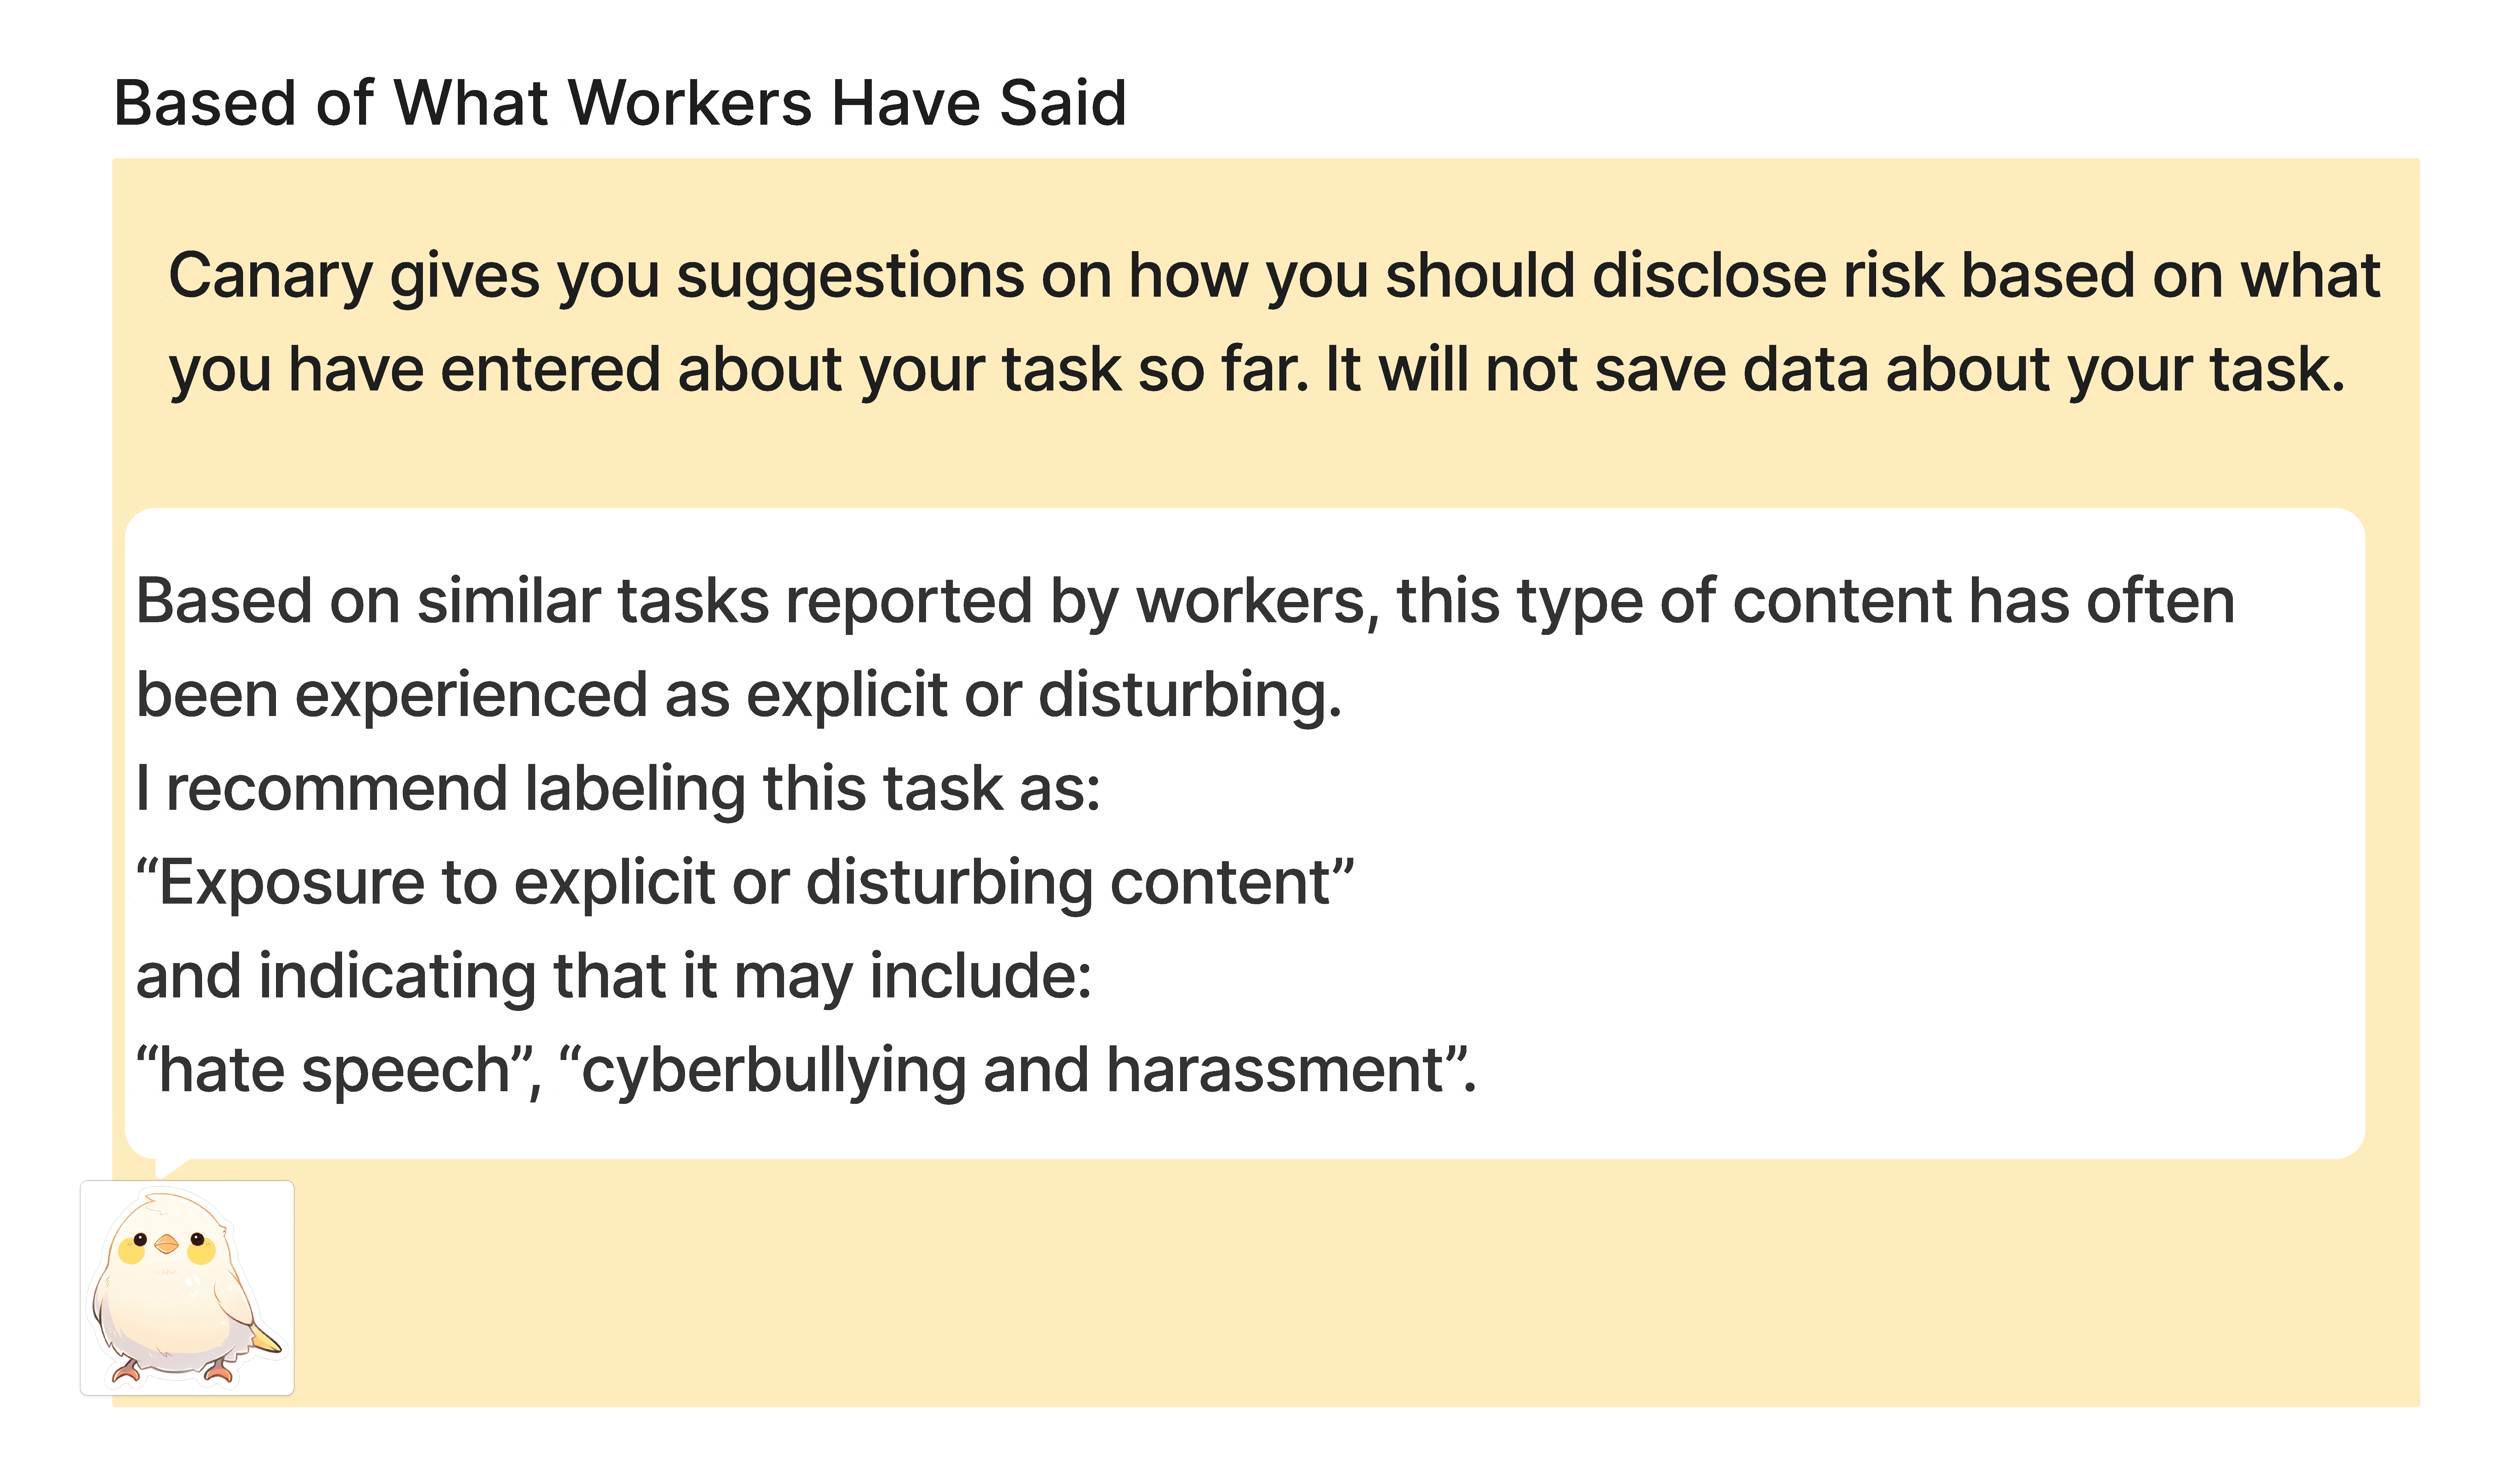
\includegraphics[width=\textwidth]{figures/study-probes/AI-probes/AI-workers.pdf} 
        \caption{Suggestion based on what workers have said}
        \label{fig:AI-based-on-workers}
    \end{subfigure}
    \caption{AI warning suggestions (Part 2)}
    \label{fig:task-designer-AI-2}
\end{figure}



\endgroup

\begin{figure}[H]
    \centering

    % First row
    \begin{subfigure}[b]{0.5\textwidth}
        \centering
        \includegraphics[width=\textwidth]{figures/study-probes/task-designer-probes/binary-task-designer.pdf}
        \caption{Binary}
        \label{fig:manual-binary}
    \end{subfigure}
    \hfill
    \begin{subfigure}[b]{0.48\textwidth}
        \centering
        \includegraphics[width=\textwidth]{figures/study-probes/task-designer-probes/keywords-task-designer.pdf}
        \caption{(Keywords}
        \label{fig:manual-keywords}
    \end{subfigure}

    \vspace{0.5em}

    % Second row
    \begin{subfigure}[b]{0.48\textwidth}
        \centering
        \includegraphics[width=\textwidth]{figures/study-probes/task-designer-probes/category-task-designer.pdf}
        \caption{Category}
        \label{fig:manual-category}
    \end{subfigure}
    \hfill
    \begin{subfigure}[b]{0.48\textwidth}
        \centering
        \includegraphics[width=\textwidth]{figures/study-probes/task-designer-probes/modality-task-designer.pdf}
        \caption{Modality}
        \label{fig:manual-modality}
    \end{subfigure}

    \vspace{0.5em}

    % Third row
    \begin{subfigure}[b]{0.48\textwidth}
        \centering
        \includegraphics[width=\textwidth]{figures/study-probes/task-designer-probes/severity-task-designer.pdf}
        \caption{Severity}
        \label{fig:manual-severity}
    \end{subfigure}
    \hfill
    \begin{subfigure}[b]{0.48\textwidth}
        \centering
        \includegraphics[width=\textwidth]{figures/study-probes/task-designer-probes/example-task-designer.pdf}
        \caption{Example}
        \label{fig:manual-example}
    \end{subfigure}
    \caption{Task designer manual options}
    \label{fig:task-designer-manual}
\end{figure}

\twocolumn[
\subsection{Additional participant demographics}\label{appendix:demographics}]
\begin{table}
\centering
\small
\begin{tabular}{p{2cm} p{5cm}}
\toprule
\textbf{Category} & \textbf{Summary} \\
\midrule
Organization type 
& Academia (4), Industry (11)\\
Organization size (number of employees)
& 10-40 (1), 50-249 (2), 1,000-4,999 (4), 5,000-24,999 (6), NA (1)\\

Task types 
& Data generation (8), Data labeling (11), Content removal (10), Adversarial prompting (6),  \\

Types of sensitive content 
& Misinformation (2), Bias\textbackslash Stereotyping (5), Hatespeech (6), Harassment and Bullying (5), Violent and graphic content (5), Terrorism and extremism (3), Self-harm and suicide (3)\\

Typical target responses per task
& < 100 responses (2), < 100 (2), < 1,000 (2), < 10,000 (7), < 100,000 (1), NA (2)\\

Platforms used 
& Prolific (10), Amazon Mechanical Turk (7), Remotasks (2), TaskUs (2) \\
\bottomrule
\end{tabular}
\caption{Summary of task designer participant characteristics across organization size, task types, sensitive content handled, target number of responses per task, and platforms used. Note that aggregate counts are not mutually exclusive, as some participants used more than one platform, for example. NA counts represent areas where participants chose not to disclose additional details.}
\label{tab:participant_summary_task_designer}
\end{table}

\begin{table}
\centering
\small
\begin{tabular}{p{2cm} p{5cm}}
\toprule
\textbf{Category} & \textbf{Summary} \\
\midrule
Task types 
& Data generation (9), Data labeling (11), Content removal (10), Adversarial prompting (7), \\

Types of sensitive content 
& Misinformation (6), Bias\textbackslash Stereotyping (6), Hatespeech (6), Harassment and Bullying (5), Violent and graphic content (6), Terrorism and extremism (1), Sexually explicit content (5), Self-harm and suicide (3), Illegal activities (2), Scams and fraud (2) \\

Typical number of tasks completed per day
& 1-10 (3), 11-50 (8), 51-100 (1) \\

Platforms used 
&  Prolific (8), Amazon Mechanical Turk (8), DataAnnotation (2), TaskUs (2)\\
\bottomrule
\end{tabular}
\caption{Summary of worker participant characteristics across task types, sensitive content handled, target number of responses per task, and platforms used. Note that aggregate counts are not mutually exclusive, as some participants used more than one platform, for example.}
\label{tab:participant_summary_worker}
\end{table}

% \color{red}